\section{Case Study}
\label{sec:case_study}

In this section, we provide a case study of magnetic control of
perturbed plasma equilibria using the HBT-EP ``Tokamak'' equiped with
the GPU and the presented I/O processing schemes.
This control system requires low latency and high computing capabilities
to achieve a sampling period of the order of ten microsenconds, while
processing 96 inputs and 64 outputs of 16-bit data with a complex
algorithm.
As mentioned in Section~\ref{sec:introduction}, the CPU implementation
of this algorithm has never met the requirement of computing power.
The case study presented herein, therefore, is signicant in that we look
into a possibility of GPU implementations for the plasma control system.

\begin{figure}[t]
 \centering
 \includegraphics[width=\hsize]{eps/tokamak_sysarch.eps}
 \caption{HBT-EP magnetic sensors and control coils connected with the
 GPU.}
 \label{fig:tokamak_sysarch}
\end{figure}

Figure~\ref{fig:tokamak_sysarch} shows a system architecture used in
this case study.
The control input comes from a set of magnetic sensors through the
D-TACQ ACQ196 digitizer, and the resulting control signal is pulled by
two D-TACQ AO32 analog output modules to excite control coils.
These input and output module devices are connected to the GPU via the
PCIe bus.
We demonstrate that our zero-copy I/O processing scheme reduces both
the algorithm cycle time and the data transfer latency of feedback
control under this system architecture.

\begin{figure}[t]
 \centering
 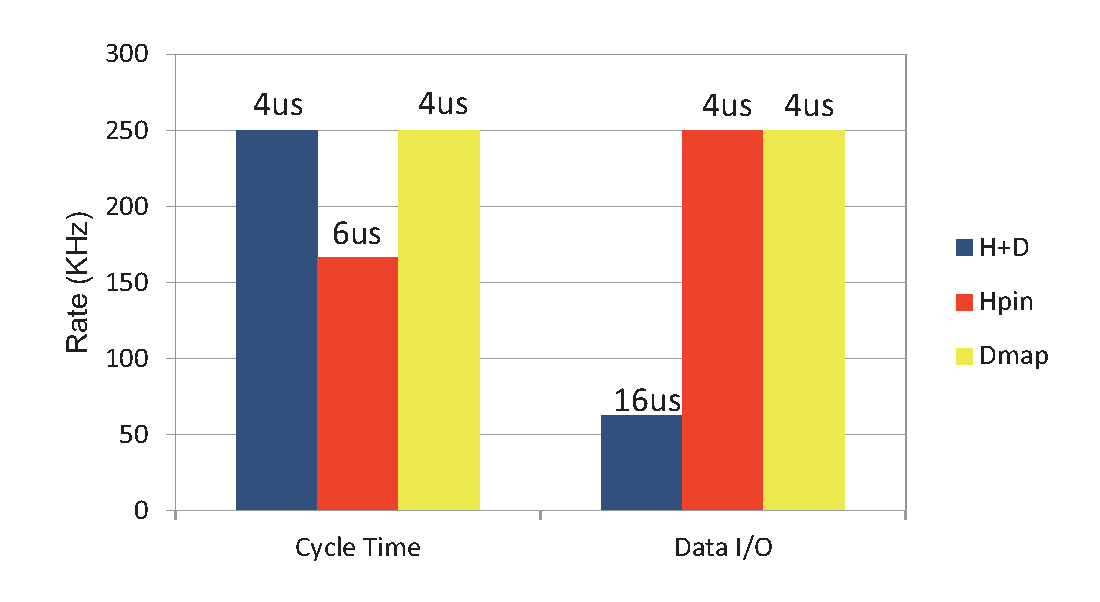
\includegraphics[width=\hsize]{eps/eval_plasma.eps}
 \caption{Cycle time and latency of feedback control using the HBT-EP
 ``Tokamak''.}
 \label{fig:eval_plasma}
\end{figure}

The cycle time and the latency of this feedback control system are shown
in Figure~\ref{fig:eval_plasma}.

\begin{figure}[t]
 \centering
 \includegraphics[width=0.85\hsize]{eps/oscilloscope.eps}
 \caption{Screenshot of the oscilloscope.}
 \label{fig:oscilloscope}
\end{figure}

\begin{figure}[t]
 \centering
 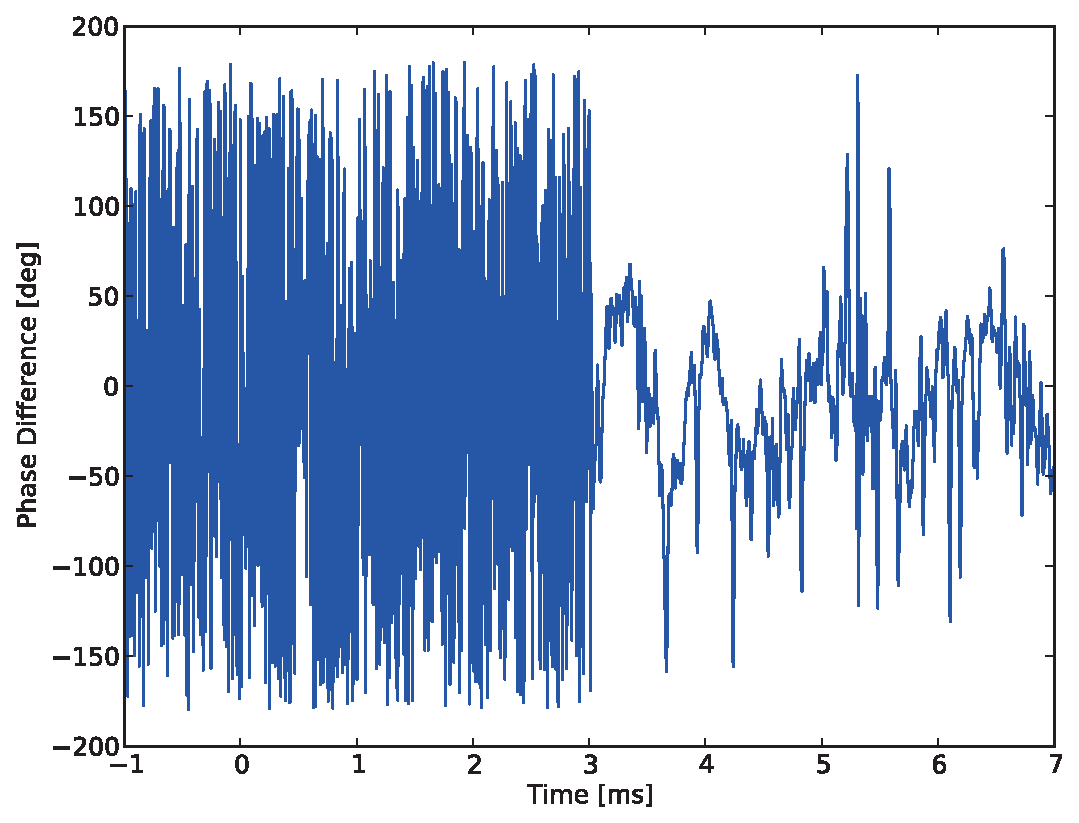
\includegraphics[width=0.7\hsize]{eps/75221_base.eps}
 \caption{Phase difference observed with the based output signal.}
 \label{fig:phase_base}
\end{figure}

\begin{figure}[t]
 \centering
 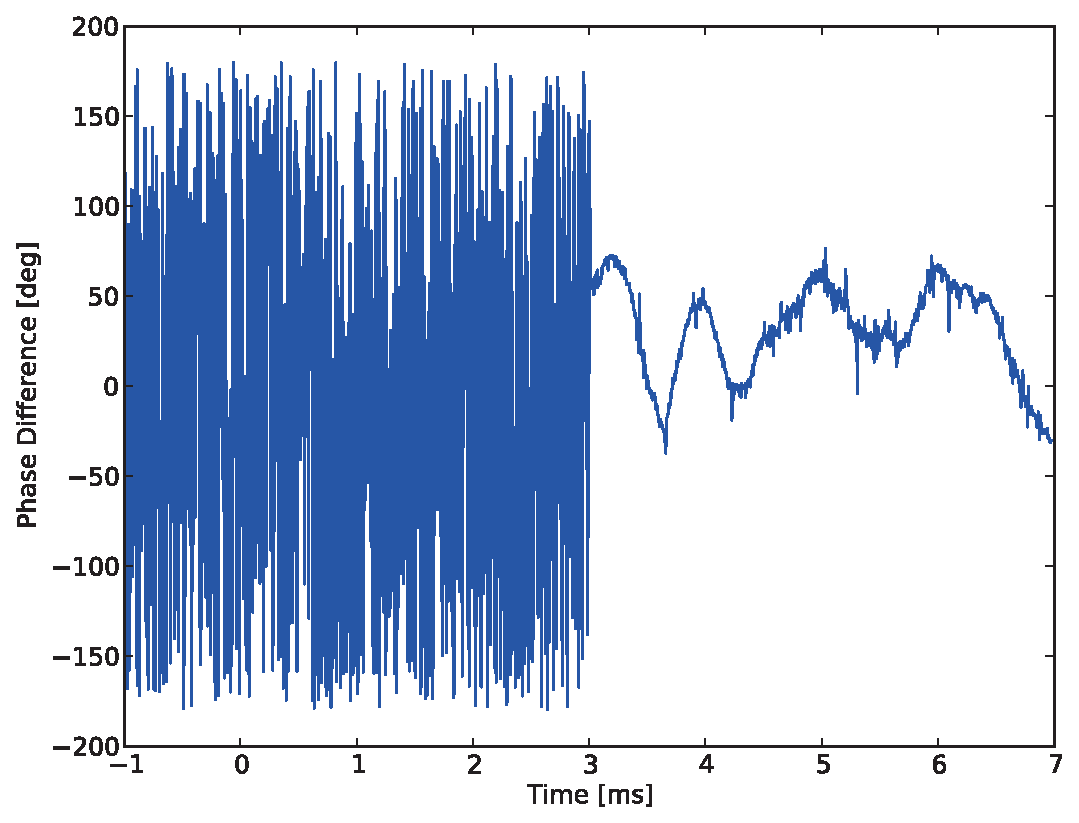
\includegraphics[width=0.7\hsize]{eps/75221_shifted.eps}
 \caption{Phase difference observed with the output signal shifted by 16$\mu$s.}
 \label{fig:phase_shifted}
\end{figure}

\begin{figure}[t]
 \centering
 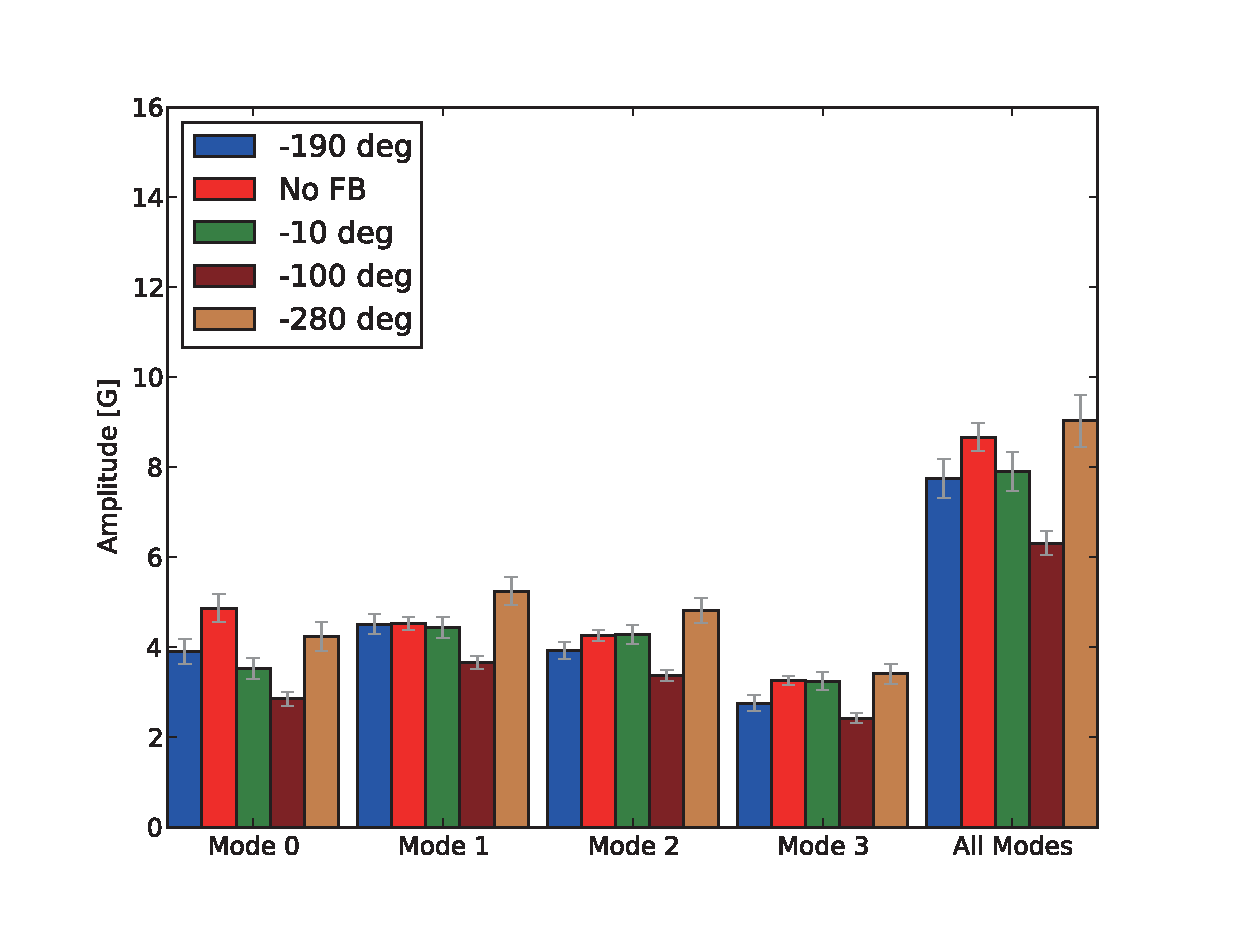
\includegraphics[width=0.9\hsize]{eps/overview.eps}
 \caption{New findings of plasma control.}
 \label{fig:plasma_overview}
\end{figure}
